\section{Interface design and documentation}

\begin{definition}[\textit{Interface}]
    An interface is a boundary where components interact. 
\end{definition}
The precise definition of interfaces carries significant architectural implications as it directly affects maintainability, usability, testability, performance, and integrability. 
Two fundamental guiding principles are information hiding and low coupling.
The key aspects to consider when designing interfaces are as follows: 
\begin{itemize}
    \item \textit{Contract principle}: any addition of a resource (operation or data) to an interface signifies a commitment to maintaining it.
    \item \textit{Least surprise principle}: interfaces should behave consistently with expectations. 
    \item \textit{Small interfaces principle}: interfaces should expose the minimum necessary resources.
\end{itemize}
When designing interfaces, we have also to define: 
\begin{itemize}
    \item \textit{Interaction style}: 
        \begin{itemize}
            \item \textit{Socket}: after connection establishment, communication is bidirectional, and both parties must agree on the same protocol.
            \item \textit{RPC/RMI}: resembles a procedure/method call in a centralized setting. 
                It requires stubs and skeletons to transform procedure/method calls into messages and vice versa.
            \item \textit{REST} (REpresentational State Transfer): this is a standardized architectural style for Application Programming Interfaces (APIs) that emphasizes clear separation between distributed, heterogeneous systems and their components.
        \end{itemize}
    \item \textit{Representation and structure of exchanged data}: the choice of data representation impacts expressiveness, interoperability, performance, and transparency.
        Common representations include XML (verbose, requires multiple parsing passes), JSON (more compact than XML, single-pass parsing), and Protocol Buffers (most compact, data passed as binary).
    \item \textit{Error handling}: possible reactions to errors include raising an exception, returning an error code, or logging the problem.
\end{itemize}
A server can offer multiple interfaces concurrently, enabling the separation of concerns, different access rights levels, and support for interface evolution.
Interfaces constitute the contract between servers and clients, and sometimes interfaces need to evolve.
The strategies used to support this continuity are: 
\begin{itemize}
    \item \textit{Deprecation}: declare in advance that an interface version will be eliminated by a certain date.
    \item \textit{Versioning}: maintain multiple active versions of the interface.
    \item \textit{Extension}: a new version extends the previous one. 
\end{itemize}

\subsection{Representational state transfer}
REST APIs are simple and standardized, alleviating developers from concerns about communication protocols (HTTP), data formatting (JSON), and request/response encoding. 
REST is stateless, which means it doesn't retain states across servers and clients, making it lightweight, scalable, and supportive of caching for high performance.

The available CRUD requests are:
\begin{itemize}
    \item \textit{Create} (HTTP POST): used to create a new resource.
    \item \textit{Read} (HTTP GET): used to retrieve an existing resource.
    \item \textit{Update} (HTTP PUT): used to modify a resource.
    \item \textit{Delete} (HTTP DELETE): used to remove a resource.
\end{itemize}
\begin{figure}[H]
    \centering
    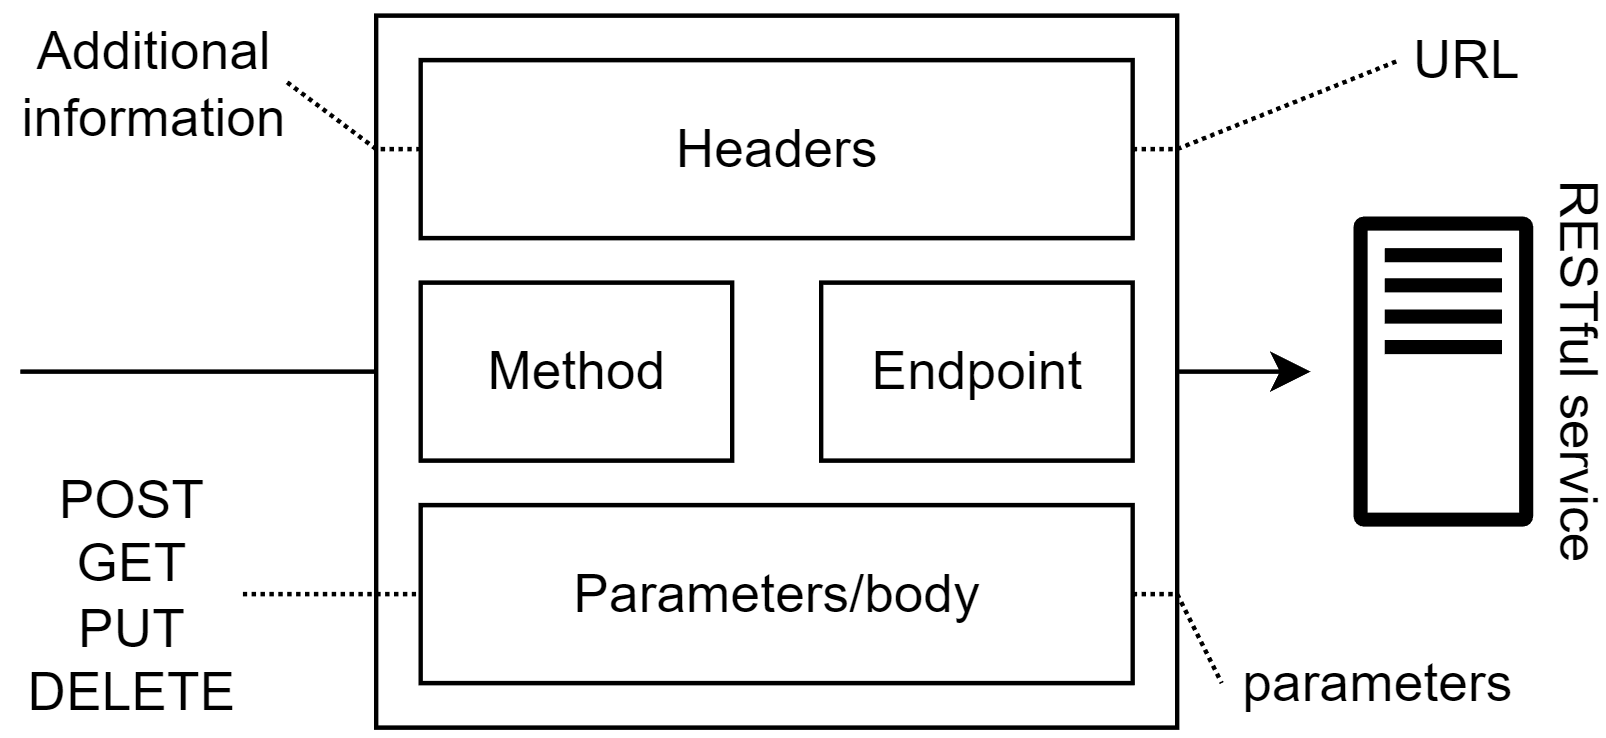
\includegraphics[width=0.6\linewidth]{images/rest.png}
    \caption{Structure of a request}
\end{figure}
\begin{figure}[H]
    \centering
    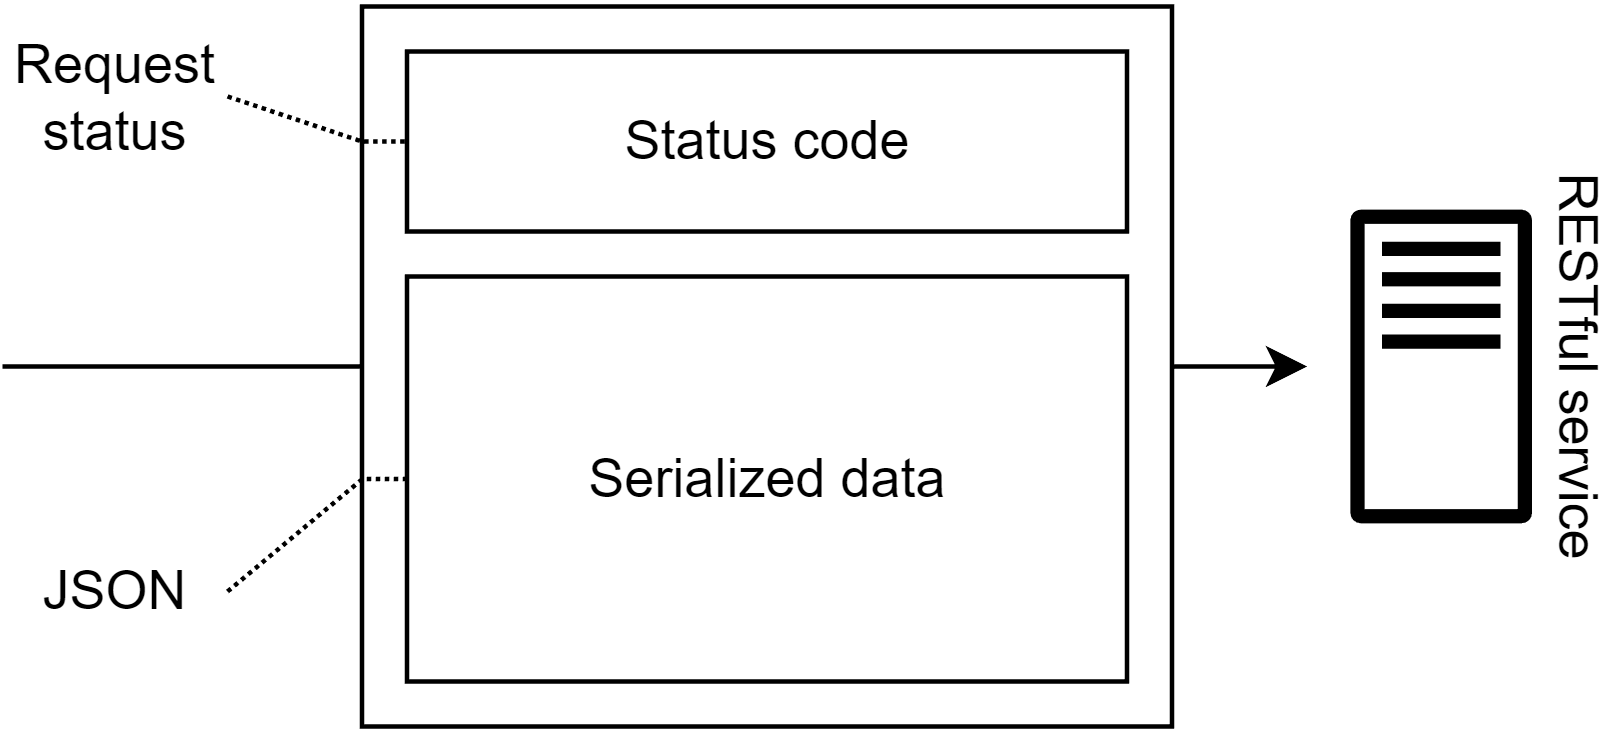
\includegraphics[width=0.6\linewidth]{images/rest1.png}
    \caption{Structure of a response}
\end{figure}

\subsection{Interface documentation}
Interface documentation explains how to use an interface without revealing details of the component's internals. 
The audience for interface documentation includes developers and maintainers of both the offering and using components, quality assurance teams for system integration and testing, and software architects seeking reusable components.

To document a REST API, the OpenAPI specification is used.
It describes a REST API interface through an OpenAPI definition, typically in JSON or YAML format.
Benefits of this type of documentation include its standardized format, public accessibility, and suitability for both human understanding and machine automation tasks like testing and code generation.

The OpenAPI definition covers endpoints, resources, operations, parameters (including data types), and authentication/authorization mechanisms. 
Support tools for OpenAPI documentation include API validators, documentation generators, and SDK generators for automated client library creation in various programming languages.